В начале семестра был переписан модуль <<Outlook>> под новую строго оформленную архитектуру <<COEX>>.
Добавлены наследуемые функции для описания плагина и функции для контроля выполнения плагина в программном комплексе <<COEX>> из главного класса <<task>> рисунок 1, рисунок 2.

Функции для описания плагина и функции для контроля выполнения плагина~\ref{Outlook:Outlook}.

\begin{figure}[h!]
\center{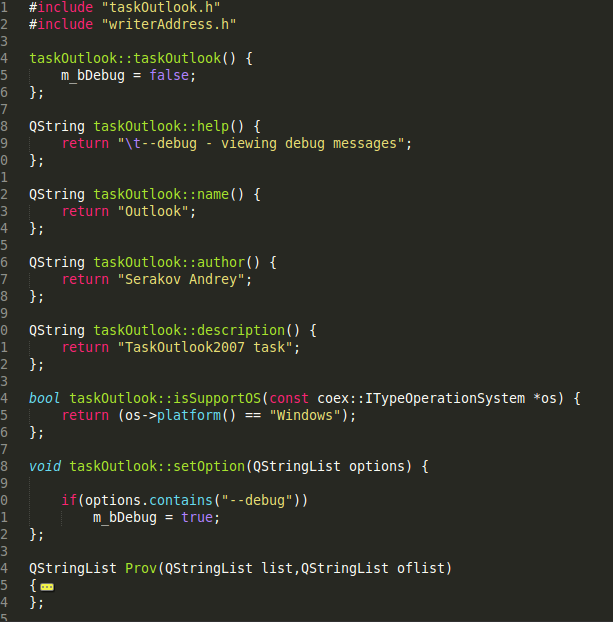
\includegraphics[width=0.6\linewidth]{Outlook}}
\caption{ Функции для описания плагина и функции для контроля выполнения плагина }
\label{Outlook:Outlook}
\end{figure}

Функция для контроля выполнения плагина в программном комплексе <<COEX>>~\ref{Outlook2:Outlook2}.

\begin{figure}[h!]
\center{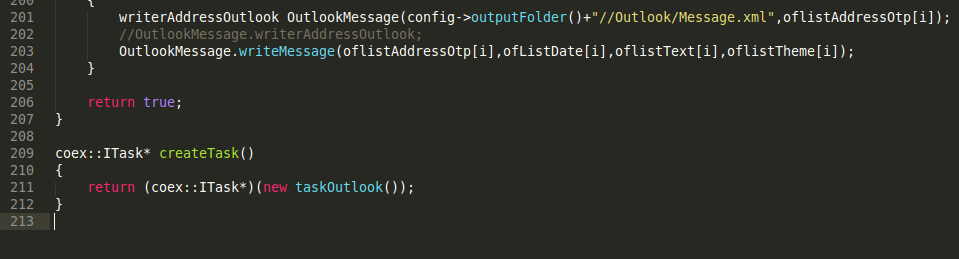
\includegraphics[width=0.6\linewidth]{Outlook2}}
\caption{ Функция для контроля выполнения плагина в программном комплексе }
\label{Outlook2:Outlook2}
\end{figure}

\subsection {Создание <<бинарного>> пакета DEB из исходных файлов программного комплекса <<COEX>>}

Для распространения и установки программного комплекса <<COEX>> был выбран <<бинарный>> формат пакета *.deb , так как он является одним из самых распространенных форматов. 

*.deb --- расширение имён файлов <<бинарных>> пакетов для распространения и установки программного обеспечения в ОС проекта Debian, и других, использующих систему управления пакетами dpkg. Пакеты Debian содержат выполняемые и конфигурационные файлы, номер версии формата, информацию об авторских правах, а также другую документацию, необходимую для установки программы из пакета.

Из чего состоит *.deb пакет, или что нужно для его создания:

\begin{enumerate}
\item control;
\item md5sums;
\item changelog;
\item rules;
\item README;
\item conffiles;
\item dirs;
\item watch.
\end{enumerate}

control --- центральный файл пакета (обязательный), описывающего все основные свойства. Файл --- текстовый, состоящий из пар <<Атрибут: значение>>.[2]

md5sums - Содержит md5 хеши для всех файлов кроме файлов находящихся в каталоге DEBIAN/. Данный файл необязателен для deb-пакета, 
однако программы верификации пакетов считают пакеты, не содержащие этот файл ошибочными. Может использоваться некоторыми программами администрирования системы для верификации изменений в файловой системе [1]. Осуществляет контроль целостности файлов.

changelog --- Это обязательный файл, его специальный формат описан в руководстве по политике Debian, раздел 4.4 <<debian/changelog>>. Этот формат используется программой dpkg и другими для получения информации о номере версии, редакции, разделе и срочности пакета [1].

rules --- используется для управления компиляцией пакета [2].

README --- в этот файл записывается любая дополнительная информация, а также различия между программой из пакета Debian и исходной программой [2].

conffiles --- Обычно пакеты содержат болванки конфигурационных файлов, например, размещаемых в /etc. Очевидно, что если конфиг в пакете обновляется, пользователь потеряет свой отредактированный конфиг. Эта проблема легко решается использованием папок типа <<config.d>>, содержимое которых включается в основной конфиг, заменяя собой повторяющиеся опции [2].

dirs --- В этом файле указываются каталоги, которые необходимы для обычной установки (make install DESTDIR=..., вызываемая dh\_auto\_install), но которые автоматически не создаются. Обычно, это указывает на проблему в Makefile [1].

watch --- Формат файла watch описан в справочной странице uscan(1). Файл watch настраивает программу uscan (предоставляется пакетом devscripts) для слежения за сайтами, с которых вы скачали исходный код. Он также используется службой Debian для слежения за состоянием внешних источников (DEHS)[1].

Для решения этой задачи было сделано:

\begin{enumerate}
\item изучен *.deb формат, особенности файлов стандартов необходимых для создания данного пакета и установки его в операционные системы семейства Unix; 
\item изучены программные продукты для работы с данным форматом (dpkg,build-essential,quilt,fakeroot,devscripts,debhelper и dh-make,lintian);
\item изучены особенности написания скриптов bash для операционных систем Unix;
\item ознакомление и изучение программы make, набора инструкцией Makefile и программной утилиты для QT C++ qmake;
\item углубленное изучение системы построения программного комплекса <<COEX>> и зависимых библиотек для компиляции данного программного комплекса;
\item создание двух программ bash-скриптов для формирования *.deb пакета и формирования changelog на основе истории коммитов системы контроля версий GIT;
\item тестирование на <<чистой>> операционной системе Linux Mint 17.2;
\item изучен формат набора макрорасширений системы компьютерной вёрстки LaTeX, личный отчет по групповому проектному обучению был оформлен согласно данному формату, и отдан документатору для редакции и включения в общий отчет.
\end{enumerate}

\subsubsection{ Подробное рассмотрение программ bash-скриптов для формирования *.deb пакета и формирования changelog}

В начале программы мы с помощью скрипта build.sh компилируем проект и получаем бинарный файл <<coex>>, а также динамические библиотеки используемые программным комплексом <<COEX>>, и исполняемый файлы плагинов данного проекта формата *.so. 

В корне пакета создается папка <<DEBIAN>>. Эта папка содержит управляющую генерацией пакета информацию, и не копируется на диск при установке пакета.
Также корневая папка пакета содержит будущий «корень диска»: при установке пакета все файлы (кроме папки <<debian>>) распаковываются в корень /. поэтому наш бинарный файл должен лежать по такому пути, относительно корня пакета: <<usr/bin/coex>>, что и было сделано в скрипте create\_package.sh рисунок 3. 

Копирования основного бинарного файла проекта~\ref{cpcoex:cpcoex}.

\begin{figure}[h!]
\center{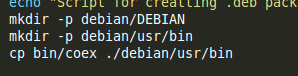
\includegraphics[width=0.6\linewidth]{cpcoex}}
\caption{Копирования основного бинарного файла проекта}
\label{cpcoex:cpcoex}
\end{figure}


Копирование исполняемых файлов плагинов данного проекта формата *.so в <<usr/bin/coex/plugins>> рисунок 4, и программных библиотек программного комплекса <<COEX>> в <<usr/bin/coex/libs>>. Для последующей установки данного программного обеспечения на компьютеры пользователей и запуска программного обеспечения <<COEX>> рисунок 5. 

Исполняемые файлы плагинов и программные библиотеки программного комплекса <<COEX>>~\ref{PluginsAndLibs:PluginsAndLibs}.

\begin{figure}[h!]
\center{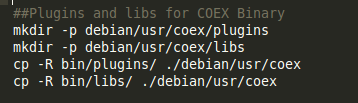
\includegraphics[width=0.6\linewidth]{PluginsAndLibs}}
\caption{Исполняемые файлы плагинов и программные библиотеки программного комплекса <<COEX>>}
\label{PluginsAndLibs:PluginsAndLibs}
\end{figure}

Установка иконки продукта, нужна если будет реализована GUI приложение для программного комплекса <<COEX>> рисунок 6. Файл coex.desktop, служит для запуска приложения, содержит основную информацию о программном комплексе <<COEX>> рисунок 7.

Иконка для GUI приложения ``COEX''~\ref{image:image}.

\begin{figure}[h!]
\center{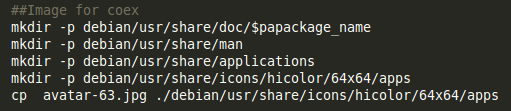
\includegraphics[width=0.6\linewidth]{image}}
\caption{ Иконка для GUI приложения ``COEX'' }
\label{image:image}
\end{figure}

Файл coex.desktop ``COEX''~\ref{Aplicatio:Aplicatio}.

\begin{figure}[h!]
\center{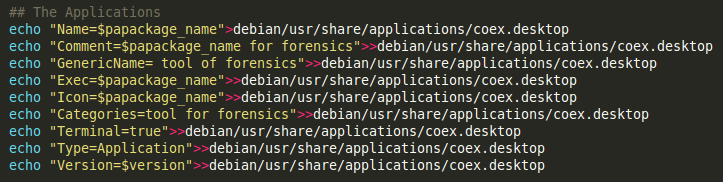
\includegraphics[width=0.6\linewidth]{Aplicatio}}
\caption{ Файл coex.desktop ``COEX'' }
\label{Aplicatio:Aplicatio}
\end{figure}

Лицензия на программный комплекс ``COEX'' защищает права разработчиков данного программного обеспечения. Мануал по использованию программного комплекса ``COEX'' находится в разработки, будет содержать основные команды при использовании программного комплекса ``COEX'', информацию о плагиннах и об особенностях работы с ними. рисунок 8

Лицензия и мануал по ``COEX''~\ref{LIcenzMan:LIcenzMan}.

\begin{figure}[h!]
\center{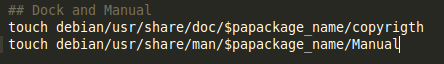
\includegraphics[width=0.6\linewidth]{LIcenzMan}}
\caption{ Лицензия и мануал по ``COEX'' }
\label{LIcenzMan:LIcenzMan}
\end{figure}

Файл control обязательный файл, в котором прописана версия программного комплекса ``COEX''. Также указаны зависимости от библиотек нужных для использования ``COEX''. Платформа на которой будет использоваться данное программное обеспечение. Рисунок 9

Файл control~\ref{control:control}.

\begin{figure}[h!]
\center{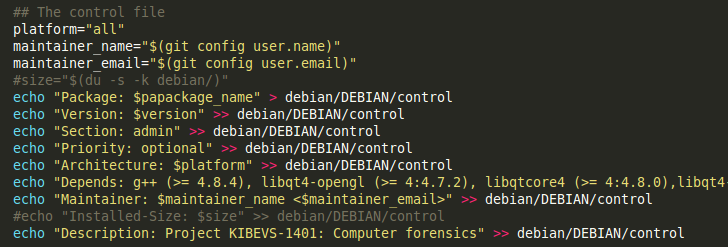
\includegraphics[width=0.6\linewidth]{control}}
\caption{ Файл control }
\label{control:control}
\end{figure}

Файл changelog в данном файле находится сведения о всех изменениях программного комплекса ``COEX'' и версий пакета, генерируется в отдельном скрипте gen\_change\_log.sh рисунок 10

Файл chengelog~\ref{chengelog:chengelog}.

\begin{figure}[h!]
\center{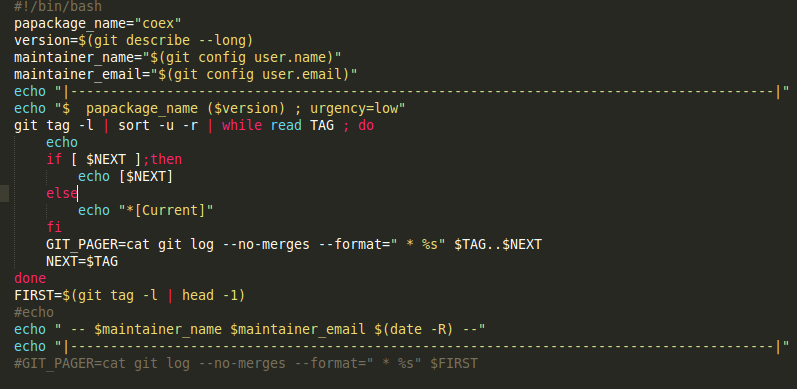
\includegraphics[width=0.6\linewidth]{chengelog}}
\caption{ Файл chengelog }
\label{chengelog:chengelog}
\end{figure}

Файл md5sums в данном файле записываются хеш значения от все файлов находящихся в ``debian/usr''. рисунок 11

Файл md5sums~\ref{md5sums:md5sums}.

\begin{figure}[h!]
\center{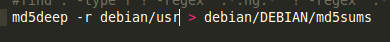
\includegraphics[width=0.6\linewidth]{md5sums}}
\caption{ Файл md5sums }
\label{md5sums:md5sums}
\end{figure}

Далее чтобы распаковать *.deb пакет для установки на компьютер пользователя нужно всем файлом дать права доступа root, иначе пакет не установится, после чего утилитой dpkg мы собираем из всех созданных файлов пакет формата *.deb. 

\subsubsection{Тестирование созданного пакета}

После создания *.deb пакета, началось его тестирование, выбраны были три образа операционных систем семейства Unix, а именно Linux Mint 17.2, Ubuntu 14.04, Debian 8.2. На каждой из операционных систем был скачен и установлен пакет coex\_0.1-43-g59b4cc1\_all.deb, программное обеспечение полностью установилось, все плагины работают. Рисунок 12-1...

Бинарный файл coex на debian~\ref{debian:debian}.

\begin{figure}[h!]
\center{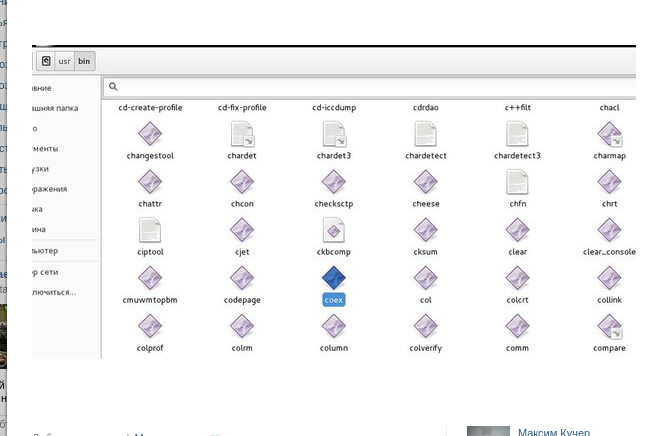
\includegraphics[width=0.6\linewidth]{debian}}
\caption{ Бинарный файл coex на debian}
\label{debian:debian}
\end{figure}

Библиотеки и исполняемый файлы плагинов coex на debian~\ref{debian2:debian2}.

\begin{figure}[h!]
\center{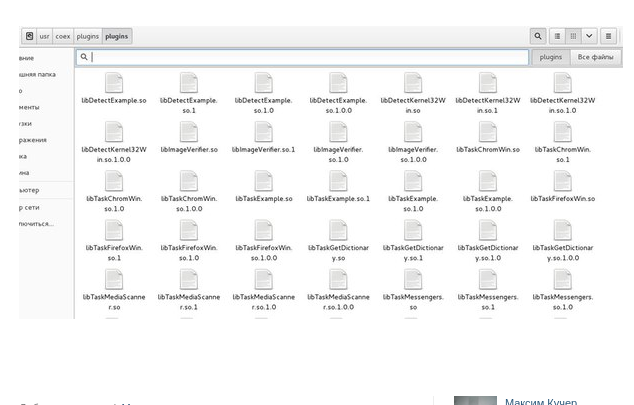
\includegraphics[width=0.6\linewidth]{debian2}}
\caption{ Библиотеки и исполняемый файлы плагинов coex на debian}
\label{debian2:debian2}
\end{figure}

Бинарный файл coex на Linux Mint~\ref{Linux Mint:Linux Mint}.

\begin{figure}[h!]
\center{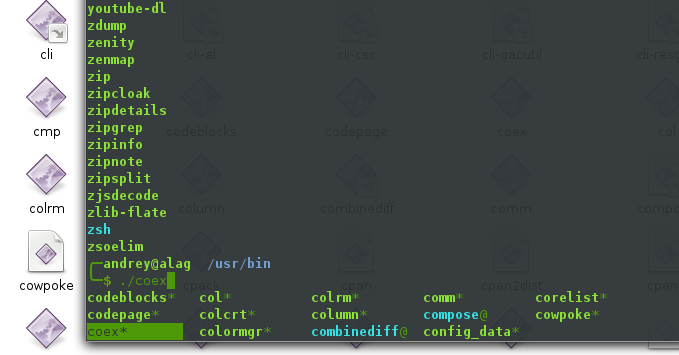
\includegraphics[width=0.6\linewidth]{Linux Mint}}
\caption{ Бинарный файл coex на Linux Mint}
\label{Linux Mint:Linux Mint}
\end{figure}

Плагины на Linux Mint~~\ref{Plugins:Plugins}.

\begin{figure}[h!]
\center{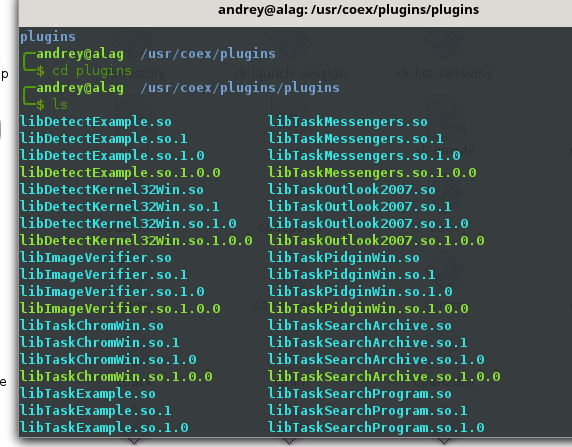
\includegraphics[width=0.6\linewidth]{Plugins}}
\caption{ Бинарный файл coex на Linux Mint}
\label{Plugins:Plugins}
\end{figure}

Запуск плагина на Linux Mint~~\ref{Zapusk:Zapusk}.

\begin{figure}[h!]
\center{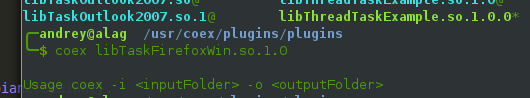
\includegraphics[width=0.6\linewidth]{Zapusk}}
\caption{ Запуск плагина на Linux Mint}
\label{Zapusk:Zapusk}
\end{figure}

\cite{deb_package_howto} 
\cite{deb_man} 

\clearpage











